\begin{minipage}{0.52\linewidth}
	Une montgolfière décolle d'un village de montagne.

	L'évolution de l'altitude de cette montgolfière en fonction du temps peut être modélisée par la fonction $f$ définie sur l'intervalle $[0 ; 5]$ par
	\[ f(t) = \dfrac{4t+1}{\mathrm{e}^t}, \]
	où $f(t)$ désigne l'altitude, en kilomètres, par rapport au niveau de la mer, et $t$ désigne le temps, en heures, écoulé depuis le décollage.
\end{minipage}
\hfill
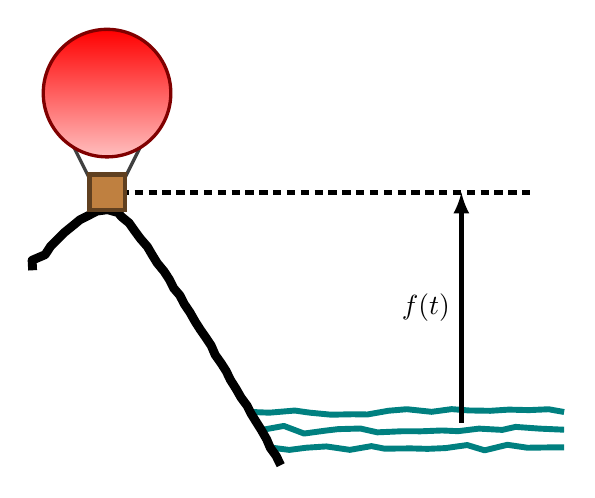
\begin{tikzpicture}[scale=0.9,baseline={(current bounding box.center)}]
	\tikzset{ondulation/.style args={#1et#2}{decorate,decoration={random steps, segment length=#1,amplitude=#2}}, ondulation/.default={1.25mm et 0.1mm}}
	
	\draw[line width=0.75mm,teal,ondulation={2.5mm et 0.5mm},line join=round] (3.1,0.75) -- (7.5,0.75);
	\draw[line width=0.75mm,teal,ondulation={2.5mm et 0.5mm},line join=round] (3.25,0.5) -- (7.5,0.5);
	\draw[line width=0.75mm,teal,ondulation={2.5mm et 0.5mm},line join=round] (3.35,0.25) -- (7.5,0.25);
	
	\draw[line width=1.125mm,ondulation,line join=round] plot[smooth] coordinates{(0,2.75)(1.25,3.5)(3.5,0)};
	
	\begin{scope}[shift={(1.05,3.6)}]
		\draw[ultra thick,densely dashed] (0,0.25) -- (6,0.25);
		\draw[ultra thick,<-,>=latex] (5,0.25) --++ (0,-3.25) node[midway,left] {$f(t)$};
		\draw[darkgray,very thick] (-0.25,0.45) --++ (-0.25,0.5);
		\draw[darkgray,very thick] (0.25,0.45) --++ (0.25,0.5);
		\draw[very thick,red!50!black,top color=red,bottom color=red!25,shade] (0,1.65) circle[radius=0.9];
		\draw[brown!50!black,ultra thick,fill=brown] (-0.25,0) rectangle++(0.5,0.5);
	\end{scope}
\end{tikzpicture}

\begin{enumerate}
	\item Déterminer l'altitude de la montgolfière au moment du décollage.
	\item On admet que la fonction $f$ est dérivable sur l'intervalle $[0 ; 5]$ et on note $f'$ sa fonction dérivée. Montrer que, pour tout réel $t$ de l'intervalle $[0 ; 5]$, on a
	\[ f'(t) = \dfrac{3-4t}{\mathrm{e}^t}. \]
	\item Étudier le signe de $f'(t)$ sur l'intervalle $[0 ; 5]$.

	En déduire que la fonction $f$ admet un maximum pour $t = \dfrac{3}{4}$.
	\item On sait que la montgolfière a décollé à 10\,h\,50.

	À quelle heure commence-t-elle à perdre de l'altitude ?
\end{enumerate}
